\documentclass[11pt,a4paper]{article}
\usepackage[margin=2.5cm]{geometry}
\usepackage{amsmath,amssymb}
\usepackage{booktabs}
\usepackage{graphicx}
\usepackage[hidelinks]{hyperref}
\usepackage[utf8]{inputenc}
\usepackage{float}
\usepackage{array}
\usepackage{caption}

\title{\textbf{Ph.D.\ Coding Exam --- Short Report}\\[4pt]
\large Production Planning with Gurobi\\[2pt]
\normalsize Computational Optimization --- PUCV}
\author{Pit Hurtado}
\date{May 2026}

\begin{document}
\maketitle
\tableofcontents
\newpage

% ==========================================================================
\section{Part A --- Base Model Implementation}
% ==========================================================================

\subsection{A.1\; Optimal Solution}

The MILP was built in Gurobi 11 exactly as stated in equations~(1)--(10).
The solver reached proven optimality in under 0.01~seconds (70 simplex
iterations after pre-solve).

\medskip
\noindent\textbf{Optimal objective value: \$7\,029.84}

\medskip
Table~\ref{tab:cost} details the cost breakdown.

\begin{table}[H]
\centering
\caption{Cost breakdown --- base model}
\label{tab:cost}
\begin{tabular}{lrr}
\toprule
Component & Cost (\$) & Share (\%) \\
\midrule
Production cost    & 4\,939.28 & 70.3 \\
Transportation     &   535.00  &  7.6 \\
Furnace activation & 1\,200.00 & 17.1 \\
Overtime           &   146.79  &  2.1 \\
Holding            &   208.77  &  3.0 \\
Back-orders        &     0.00  &  0.0 \\
\midrule
\textbf{Total}     & \textbf{7\,029.84} & 100.0 \\
\bottomrule
\end{tabular}
\end{table}

Table~\ref{tab:production} reports $D_{k,t}$, total production
$X_{k,t}=\sum_m x_{m,k,t}$, total delivery $Y_{k,t}=\sum_j y_{j,k,t}$,
end-of-period inventory $I_{k,t}$, and back-order $B_{k,t}$.

\begin{table}[H]
\centering
\caption{Production, delivery, inventory, and back-order plan}
\label{tab:production}
\small
\begin{tabular}{ccrrrrr}
\toprule
$k$ & $t$ & $D_{k,t}$ & $X_{k,t}$ & $Y_{k,t}$ & $I_{k,t}$ & $B_{k,t}$ \\
\midrule
A & 1 & 55 & 82.53 & 55.00 & 27.53 & 0.00 \\
A & 2 & 57 & 61.90 & 57.00 & 32.43 & 0.00 \\
A & 3 & 61 & 46.43 & 61.00 & 17.86 & 0.00 \\
A & 4 & 63 & 45.14 & 63.00 & 0.00  & 0.00 \\
\midrule
B & 1 & 36 & 63.27 & 36.00 & 27.27 & 0.00 \\
B & 2 & 39 & 47.45 & 39.00 & 35.72 & 0.00 \\
B & 3 & 52 & 35.59 & 52.00 & 19.31 & 0.00 \\
B & 4 & 46 & 26.69 & 46.00 & 0.00  & 0.00 \\
\midrule
C & 1 & 24 & 36.11 & 24.00 & 12.11 & 0.00 \\
C & 2 & 36 & 38.87 & 36.00 & 14.98 & 0.00 \\
C & 3 & 31 & 29.15 & 31.00 & 13.14 & 0.00 \\
C & 4 & 35 & 21.86 & 35.00 & 0.00  & 0.00 \\
\bottomrule
\end{tabular}
\end{table}

The optimizer adopts a \emph{produce-ahead} strategy: production in periods
1--2 exceeds current demand to build inventory that covers the higher demand
in periods 3--4.  No back-orders are ever incurred (service level $\geq 60\%$
is met by delivering 100\% of demand each period).

\medskip
Table~\ref{tab:furnace} shows the furnace activation and hour usage.

\begin{table}[H]
\centering
\caption{Furnace schedule}
\label{tab:furnace}
\begin{tabular}{cccrr}
\toprule
Furnace & $t$ & $z_{m,t}$ & Reg.\ hrs used & OT hrs \\
\midrule
F1 & 1 & 1 & 50.00 & 0.00 \\
F1 & 2 & 1 & 50.00 & 0.00 \\
F1 & 3 & 1 & 50.00 & 9.79 \\
F1 & 4 & 1 & 50.00 & 0.00 \\
\midrule
F2 & 1 & 1 & 50.00 & 0.00 \\
F2 & 2 & 1 & 29.71 & 0.00 \\
F2 & 3 & 0 & ---   & ---  \\
F2 & 4 & 0 & ---   & ---  \\
\bottomrule
\end{tabular}
\end{table}

F1 runs at full regular capacity in all periods, with a small overtime usage
in period 3 (9.79 hrs).  F2 is activated only in periods 1 and 2.

% --------------------------------------------------------------------------
\subsection{A.2\; Holding-Cost Sensitivity}

Figure~\ref{fig:alpha} plots total cost and total end-of-period inventory
$\sum_{k,t}I^*_{k,t}$ against $\alpha\in[0,5]$ (25 points).

\begin{figure}[H]
\centering
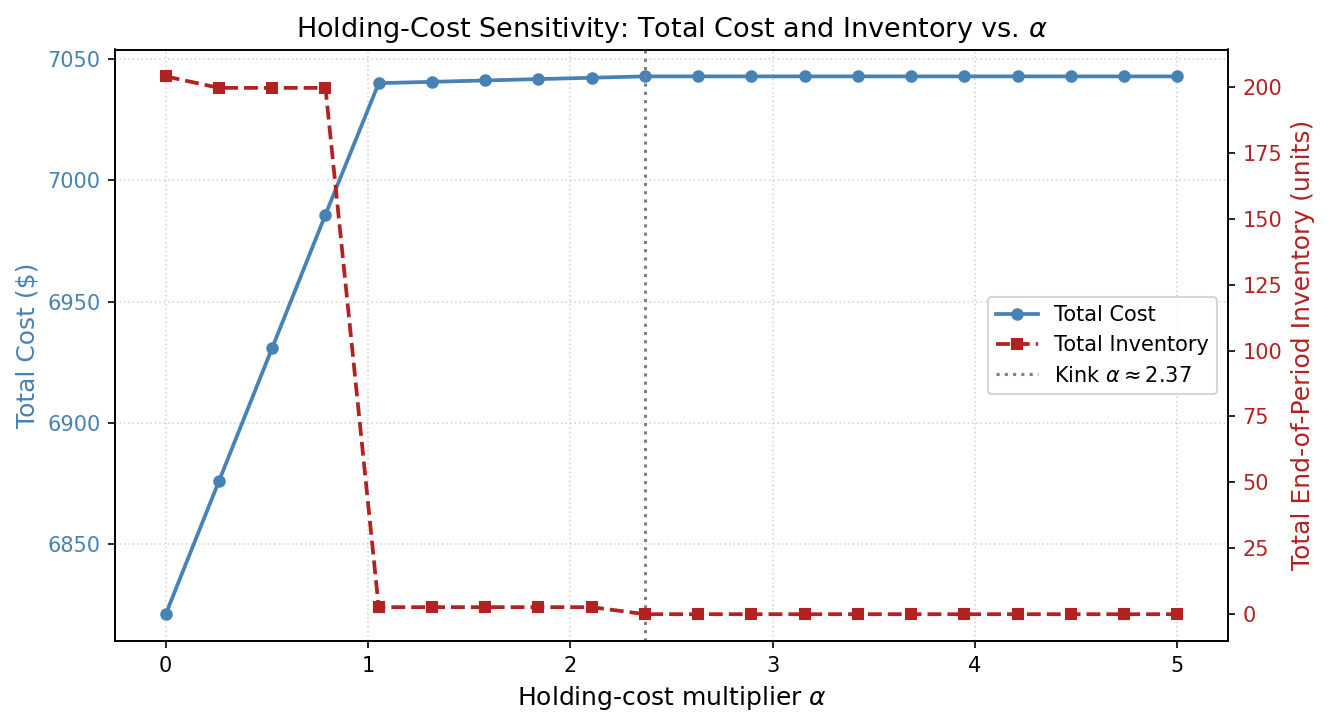
\includegraphics[width=0.88\textwidth]{fig_A2_holding_sensitivity.png}
\caption{Total cost (left axis) and total inventory (right axis) vs.\
         holding-cost multiplier $\alpha$.}
\label{fig:alpha}
\end{figure}

For $\alpha < 1.25$ the model maintains $\sim 200$ units of total inventory
(produce-ahead).  Between $\alpha=1.04$ and $\alpha=1.25$ inventory drops
sharply to $\sim 2.67$ units (the first prominent kink), and at
$\alpha \approx 2.50$ inventory falls to zero (produce-ahead strategy fully
abandoned).  Above this point the total cost plateaus at \$7\,042.92.

% --------------------------------------------------------------------------
\subsection{A.3\; Overtime-Cost Sensitivity}

Figure~\ref{fig:beta} plots total cost and total overtime hours
$\sum_{m,t}o^*_{m,t}$ against $\beta\in[0.5,4.0]$ (20 points).

\begin{figure}[H]
\centering

\includegraphics[width=0.88\textwidth]{fig_A3_overtime_sensitivity.png}
\caption{Total cost (left axis) and overtime hours (right axis) vs.\
         overtime-cost multiplier $\beta$.}
\label{fig:beta}
\end{figure}

The \textbf{breakeven} is at $\beta \approx 1.42$.  At this value the
effective overtime rate is $1.42\times\$15 = \$21.3$/hr.  Above this
threshold the optimizer eliminates overtime entirely, accepting a slightly
different production schedule instead.  Economically, $\beta=1.42$ is the
point at which paying for one hour of overtime (to produce extra units now)
is no longer cheaper than the alternative --- rearranging production across
periods while staying within regular capacity and smoothing bounds, which
raises the cost floor to \$7\,065.18.

% --------------------------------------------------------------------------
\subsection{A.4\; Discussion}

\paragraph{1.\;Why does the holding-cost curve show a clear kink?}
The kink arises because the decision to keep a furnace \emph{on} in early
periods (to build inventory) is governed by a binary variable $z_{m,t}\in
\{0,1\}$.  Below $\alpha\approx 1.25$ the optimizer finds it worthwhile to
activate F2 in periods 1--2, pre-produce $\sim 200$ units, and hold them at
cost $\alpha\cdot CH_k$.  As $\alpha$ increases, at some threshold the total
holding penalty exceeds the savings from keeping F2 active; the model then
switches to a near-just-in-time plan and cuts inventory from $\sim 200$ to
$\sim 2.67$ units in a single step.  This discrete binary switch is the
source of the sharp kink rather than a smooth, gradual slope.

\paragraph{2.\;Is furnace F2 active in all periods?}
No.  F2 is activated only in periods $t=1$ and $t=2$; it is kept off in
periods 3 and 4.  The reason is economics: F2 has a higher base production
cost ($c_0^{F2}=10$ vs.\ $c_0^{F1}=8$) plus an activation fee of \$200.  In
period 3, peak demand is high, but the smoothing constraint limits production
to at most $1.25\times X_{k,2}$; consequently, the extra units the model
would want to produce on F2 are bounded anyway.  F1 with modest overtime
(9.79 hrs) covers period~3 demand, and period~4 demand is met from F1 plus
the inventory buffer built in periods 1--2.  Keeping F2 off in periods 3--4
saves \$400 in activation costs.

\paragraph{3.\;Role of the smoothing constraints.}
Constraints (9)--(10) bound $X_{k,t}$ to within $\pm 25\%$ of $X_{k,t-1}$,
coupling all time periods.  They prevent \emph{bang-bang} policies in which
the optimizer concentrates all production in the cheapest single period,
stores massive inventory, and then goes idle.  Without them, the optimal plan
would likely activate one furnace for one period (minimum activation cost),
produce everything at once, and back-order or store freely.  The smoothing
bounds force a gradual production profile that mirrors real operational
constraints on furnace scheduling and supply-chain planning.

\newpage
% ==========================================================================
\section{Part B --- Minimum Lot Size and Setup Cost}
% ==========================================================================

\subsection{B.1\; Mathematical Formulation}

\paragraph{New binary decision variables.}
\begin{equation*}
  \delta_{m,k,t} \in \{0,1\}, \quad \forall\,m\in M,\;k\in K,\;t\in T.
\end{equation*}
$\delta_{m,k,t}=1$ if and only if furnace $m$ performs a production run of
product $k$ in period $t$ (i.e.\ a setup is executed); $\delta_{m,k,t}=0$
otherwise.

\paragraph{Coupling inequalities.}
\begin{align}
  x_{m,k,t} &\leq M_{m,k,t}\;\delta_{m,k,t},
  \qquad \forall\,m,k,t \tag{B1}\label{eq:bigM}\\[4pt]
  x_{m,k,t} &\geq L_k\;\delta_{m,k,t},
  \qquad \forall\,m,k,t \tag{B2}\label{eq:minlot}
\end{align}
\begin{itemize}
  \item \textbf{Big-$M$ side \eqref{eq:bigM}:} forces $x_{m,k,t}=0$ when
    $\delta_{m,k,t}=0$ (no production without a setup).
    $M_{m,k,t}=(H_{m,t}+H^{\mathrm{ov}}_{m,t})/a_{m,k}$ is the physical
    upper bound on production (all available hours devoted to one product).
    Numerically: $M_{m,A,t}=140$, $M_{m,B,t}=100$, $M_{m,C,t}=175$.
  \item \textbf{Minimum-lot side \eqref{eq:minlot}:} forces
    $x_{m,k,t}\geq L_k$ when $\delta_{m,k,t}=1$, ensuring that every active
    production run meets the minimum lot size.
    $L_A=25$, $L_B=20$, $L_C=15$.
\end{itemize}

\paragraph{Modified objective.}
Equation (1) is extended with setup costs:
\[
  \min\;\text{(all terms of eq.\ (1))}\;
  +\;\underbrace{\sum_{m\in M}\sum_{k\in K}\sum_{t\in T}
     SC_{m,k}\;\delta_{m,k,t}}_{\text{setup costs}},
     \quad SC_{m,k}=50\;\forall\,(m,k).
\]

% --------------------------------------------------------------------------
\subsection{B.2\; Implementation and Comparison}

\begin{table}[H]
\centering
\caption{Key metrics: Part~A vs.\ Part~B}
\begin{tabular}{lrr}
\toprule
Metric & Part A & Part B \\
\midrule
Optimal objective (\$) & 7\,029.84 & 7\,637.39 \\
Cost increase (\$)     & ---       & $+607.56$ \\
Setups paid            & ---       & 12        \\
\bottomrule
\end{tabular}
\end{table}

The 12 active setups are:
$\delta_{F1,A,t}$ ($t=1,2,3,4$),
$\delta_{F1,B,t}$ ($t=3,4$),
$\delta_{F1,C,t}$ ($t=1,2,3,4$), and
$\delta_{F2,B,t}$ ($t=1,2$).

Table~\ref{tab:comparison} compares aggregate production
$X_{k,t}=\sum_m x_{m,k,t}$ under both models.

\begin{table}[H]
\centering
\caption{Aggregate production comparison $X_{k,t}$: Part~A vs.\ Part~B}
\label{tab:comparison}
\small
\begin{tabular}{ccrrr}
\toprule
$k$ & $t$ & $X^{(A)}_{k,t}$ & $X^{(B)}_{k,t}$ & $\Delta$ \\
\midrule
A & 1 & 82.53 & 74.09 & $-8.44$\;\textbf{*} \\
A & 2 & 61.90 & 67.14 & $+5.24$\;\textbf{*} \\
A & 3 & 46.43 & 50.35 & $+3.93$\;\textbf{*} \\
A & 4 & 45.14 & 44.42 & $-0.73$\;\textbf{*} \\
\midrule
B & 1 & 63.27 & 63.27 & $\phantom{+}0.00$ \\
B & 2 & 47.45 & 47.45 & $\phantom{+}0.00$ \\
B & 3 & 35.59 & 35.59 & $\phantom{+}0.00$ \\
B & 4 & 26.69 & 26.69 & $\phantom{+}0.00$ \\
\midrule
C & 1 & 36.11 & 32.39 & $-3.73$\;\textbf{*} \\
C & 2 & 38.87 & 40.48 & $+1.61$\;\textbf{*} \\
C & 3 & 29.15 & 30.36 & $+1.21$\;\textbf{*} \\
C & 4 & 21.86 & 22.77 & $+0.91$\;\textbf{*} \\
\bottomrule
\end{tabular}
\par\smallskip
\textbf{*} indicates a changed value; bold values highlight the most notable
shift in production pattern.
\end{table}

The most notable change is for product~A in period~1: $X_{A,1}$ drops from
82.53 to 74.09.  In Part~A, the model split A production between F1 and F2
($x_{F2,A,1}=11.42$); since $11.42 < L_A = 25$, this lot is infeasible in
Part~B and is eliminated, consolidating all A production onto F1.  For
product~B, the small F1 lot in period~2 ($x_{F1,B,2}=5.00 < L_B=20$)
is similarly eliminated and absorbed by F2.

% --------------------------------------------------------------------------
\subsection{B.3\; Discussion}

\paragraph{1.\;Why does Part~B cost exceed Part~A?}
There are two distinct sources.
\begin{enumerate}
  \item \textbf{Direct setup fees:} 12 setups $\times$ \$50 $=$ \$600.
  \item \textbf{Production quantity distortions:} the minimum-lot constraint
    forces the model to eliminate small lots (e.g.\ $x_{F2,A,1}=11.42$
    becomes zero) and redistribute production to other furnace--period
    combinations.  Because smoothing constraints propagate these changes
    across all subsequent periods, the resulting plan is less efficient in
    terms of inventory build-up and per-unit costs, adding the remaining
    \$7.56 above the \$600 setup fees.
\end{enumerate}

\paragraph{2.\;Would a very large $SC_{m,k}$ reduce the number of setups?}
Not necessarily to zero.  The demand constraint $B_{k,|T|}=0$ with
$I^0_k=0$ requires that every unit of demand be produced during the horizon.
With positive demand in every period and a smoothing bound of $\pm 25\%$, the
optimizer cannot concentrate all production into a single period: starting
from a non-zero $X_{k,1}$, each subsequent period must produce at least
$0.75^{t-1}\,X_{k,1}$, preventing idle periods (which would force a complete
stop followed by a restart).  In this instance the two F2-B setups
($t=1,2$) are \emph{hard-capacity forced}: F1 is fully utilized making A
and C in those periods, leaving no machine hours for B.  Even with
$SC_{m,k}\to\infty$, those setups cannot be eliminated; the model is
compelled to produce B on F2 regardless of the setup penalty.

\end{document}
